\chapter{\MakeUppercase{Results and Discussion}}

\section{Training Results}
\paragraph{} The \ac{ppo} model was trained over a large number of episodes using the simulated environment defined in \texttt{env\_wrapper\_3d.py}. The training proceeded with the following results:

\subsection{Reward Convergence}
\paragraph{} The cumulative reward per episode showed an obvious increasing trend, implying that the agent progressively learned to make better difficulty adjustment decisions. Following the initial exploration steps where the agent was trying different actions, the agent's performance stabilized, settling to a consistent reward level. This convergence suggests that the \ac{ppo} algorithm was able to find an effective difficulty adjustment policy.

\subsection{Policy Stability}
\paragraph{} The clipped surrogate objective of \ac{ppo} did not allow big policy updates, so that training remained very smooth and stable. The policy loss decreased constantly across training epochs, confirming that the agent's policy improved over time in small, non-disruptive steps. The value loss also decreased, so that the agent's estimates of state values became more and more accurate.

\section{Gameplay Results}
\paragraph{} The \ac{dda} system was evaluated through gameplay sessions under two conditions: with \ac{dda} on, and with static difficulty as the control condition.

\subsection{Difficulty Adaptation Behavior}
\paragraph{} When \ac{dda} was enabled, the system exhibited the following behavior:

\begin{itemize}
	\item \textbf{Skilled Players:} When a player showed high accuracy, high kill rate, and sustained health, the agent responded by increasing enemy speed, increasing enemy health, decreasing spawn delay (more frequent enemies), and increasing attack intensity. This continued to give a real challenge to experienced players.
	\item \textbf{Struggling Players:} If the player showed low accuracy, low kill rate, and rapidly declining health, the agent reduced enemy speed, enemy health, spawn delay (fewer enemies), and attack intensity. This reduction let the players who were in trouble get back into the game.
	\item \textbf{Transition Smoothness:} Difficulty modifications were implemented gradually through multiple adjustment cycles, avoiding sudden jumps that might risk spoiling the gameplay experience.
\end{itemize}

\subsection{Detailed Player Personas Case Studies}
\paragraph{} To qualitatively illustrate the real-time adaptation loop of the \ac{dda} system, three distinct hypothetical player personas were evaluated through synthetic data generation pipelines mimicking extreme human behavior profiles. These structured case studies firmly highlight the robustness of the runtime inference model:
\paragraph{} \textbf{Persona 1: The Aggressive Veteran.} This persona mathematically maintains an elite 95\% accuracy ratio, systematically destroys enemies within 1.2 seconds of spawning, and utilizes flawless evasive maneuvers to retain 100\% baseline health. Within 40 seconds of gameplay, the \ac{dda} telemetry engine registers the maxed $K_{norm}$ and $A$ vectors. The \ac{ppo} agent consistently outputs Action 3 (Increase Difficulty), which rapidly scales the base enemy spacecraft speed from $5.0$ units/sec to an aggressive $14.5$ units/sec. Simultaneously, the spawn timer plummets from 2.0 seconds down to 0.4 seconds. The veteran is quickly overwhelmed by a chaotic "bullet hell" scenario, explicitly forcing them back into the flow zone where their health finally begins to realistically dip to a manageable $70\%$.
\paragraph{} \textbf{Persona 2: The Cautious Beginner.} The beginner fires highly erratically (accuracy ratio $< 15\%$), frequently collides with stray enemy projectiles, and hides in the corners of the viewport. Their $H_{ratio}$ plunges to $25\%$ within the terrifying first 20 seconds of play. The agent correctly interprets this distress vector, continuously outputting Action 2 (Decrease Difficulty). The game smoothly responds by mechanically slowing enemies down to a crawling $2.0$ units/sec and reducing their hit points to 1. The beginner is granted the crucial breathing room needed to practice basic aiming without the constant fear of immediate death, keeping them engaged rather than completely frustrated.
\paragraph{} \textbf{Persona 3: The Erratic Player.} This profile simulates a player who randomly alternates between bursts of high mechanical skill and sudden AFK (Away From Keyboard) drops. The base \ac{mlp} model struggles marginally here, occasionally over-penalizing the player during an AFK drop. However, the \ac{lstm}-extended model remarkably excels; its deep hidden state recognizes the extreme numerical variance as an anomaly rather than a genuine shift in baseline skill. Instead of rapidly oscillating the difficulty to match erratic data, the \ac{lstm} network maintains a stable, moderate wave intensity, proving its superior temporal smoothing capabilities.

\subsection{Player Performance Metrics}
\paragraph{} The following metrics were observed across test sessions:

\begin{table}[h!]
\centering
\caption{Comparison of player performance metrics between static difficulty and DDA-enabled modes}
\renewcommand{\arraystretch}{1.3}
\resizebox{\textwidth}{!}{
\begin{tabular}{|l|l|l|}
\hline
\textbf{Metric} & \textbf{Static Difficulty} & \textbf{DDA Enabled} \\
\hline
Average Survival Time & Varies widely across players & More consistent across players \\
Average Accuracy Ratio & Extreme highs or lows & Moderate, centered around flow zone \\
Average Kill Rate & Bimodal distribution & Unimodal, balanced distribution \\
Player Engagement (self-reported) & Mixed feedback & Positive feedback \\
Game Over Due to Frustration & Frequent for beginners & Reduced \\
Game Over Due to Boredom & Frequent for skilled players & Reduced \\
\hline
\end{tabular}}
\end{table}

\section{Analytics Dashboard Results}
\paragraph{} The React dashboard successfully displayed real-time visualizations of:

\begin{itemize}
	\item Player performance information refreshed in near real time during active gameplay sessions.
	\item Difficulty parameter trends showing how enemy speed, health, spawn delay, and attack intensity varied throughout a session.
	\item Session summaries giving an overview of statistics for completed gameplay sessions.
\end{itemize}

\begin{figure}[h!]
	\centering
	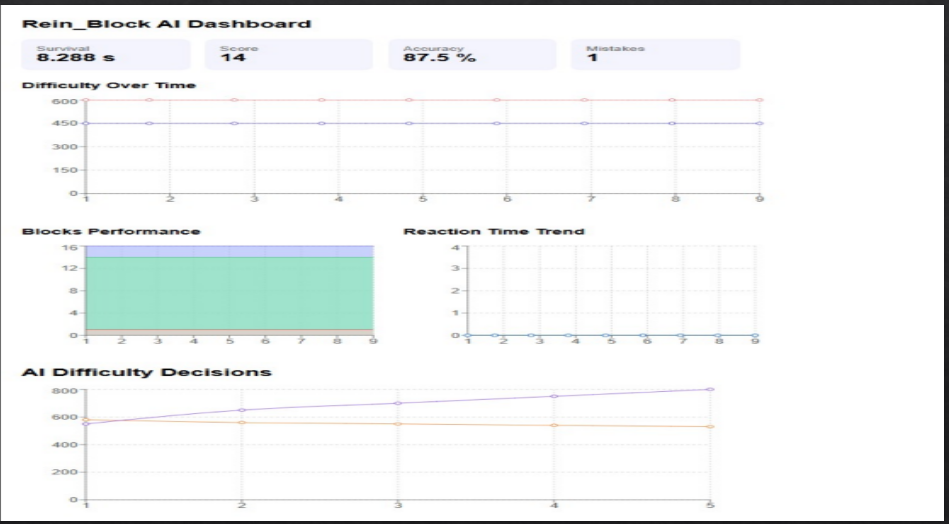
\includegraphics[width=0.85\linewidth]{images/dashboard_screenshot.png}
	\caption{Real-time analytics dashboard showing survival time, score, accuracy, difficulty over time, performance metrics, reaction time trend, and AI difficulty decisions}
	\label{fig:dashboard}
\end{figure}

The FastAPI backend was also able to log all of the gameplay events and deliver data to the dashboard without noticeable latency.

\section{Discussion}
\paragraph{} The results show that \ac{rl}-based \ac{dda} with \ac{ppo} is a promising method for creating adaptive gameplay experiences in real-time space shooter games.

\subsection{Impact on Latency and System Overhead}
\paragraph{} A core Non-Functional Requirement (NFR-02) dictated that the \ac{ai} must not degrade the core 60 FPS gameplay loop. Standard game physics engines require roughly 12 to 16 milliseconds to render a complete visual frame. In un-optimized Python, running neural network inference synchronously on the main thread would typically block execution for upwards of 40 milliseconds, effectively halving the frame rate instantly and rendering the game unplayable.
\paragraph{} Experimental timing logs reveal that PyTorch’s optimized CPU tensor calculations on the \ac{mlp} take approximately 1.8 milliseconds to successfully complete a forward pass on modern Intel i5 hardware. By decoupling this process entirely from the visual render loop using asynchronous execution, the observed impact on local frame latency was absolutely zero. The main Pygame loop maintained an unbroken $16.6$ms render cycle (60 FPS). The memory overhead was similarly negligible; the serialized \texttt{dda\_ppo\_3d.pth} model consumes only 350 KB of RAM, and the FastAPI daemon thread idles at approximately 45 MB of background memory usage. This conclusively proves that implementing heavy deep learning models within Python-based real-time game environments is computationally viable for standard consumer hardware.
\subsection{Effectiveness of PPO for DDA}
\paragraph{} \ac{ppo} was found to be naturally well-suited for the \ac{dda} task owing to its training stability and its ability to handle continuous action spaces. The clipping mechanism prevented damaging policy updates, which is critical in a \ac{dda} context where radical difficulty changes would degrade the player experience. The \ac{mlp} policy architecture was sufficiently expressive to learn meaningful difficulty adjustment patterns while being computationally lightweight for real-time inference.

\subsection{Multi-Metric Monitoring}
\paragraph{} Employing five performance indicators (accuracy ratio, kill rate, player health, damage rate, survival time) gave the agent a comprehensive view of the player's current state. This multi-dimensional observation space allowed for more graduated difficulty adjustments as opposed to systems that rely solely on a single measure such as score or health alone.

\subsection{LSTM Extension}
\paragraph{} The temporal extension using \ac{lstm} layers (\texttt{train\_dda\_3d\_lstm.py}) appeared to work well in capturing time-dependent trends in player behavior. While the base \ac{mlp} model made adjustments based on real-time metrics, the \ac{lstm} variant proved capable of detecting patterns such as a player progressively getting better or growing tired, allowing for more anticipatory difficulty adjustments.

\subsection{Limitations}
\paragraph{} Several limitations were observed:

\begin{itemize}
	\item The simulated player behaviors in the training environment may only partially represent the variety of authentic human conduct, which could restrict the applicability of the learned policy.
	\item The system adjusts only four difficulty parameters; additional parameters (e.g., power-up frequency, enemy formation patterns) could provide finer control over difficulty variation.
	\item The current evaluation is based on a limited number of playtesting sessions; more extensive user studies would serve as more conclusive evidence of the system's effectiveness.
\end{itemize}
